\begin{frame}[plain]
  \begin{tikzpicture}[remember picture,overlay]
    \node[at=(current page.center)] {
      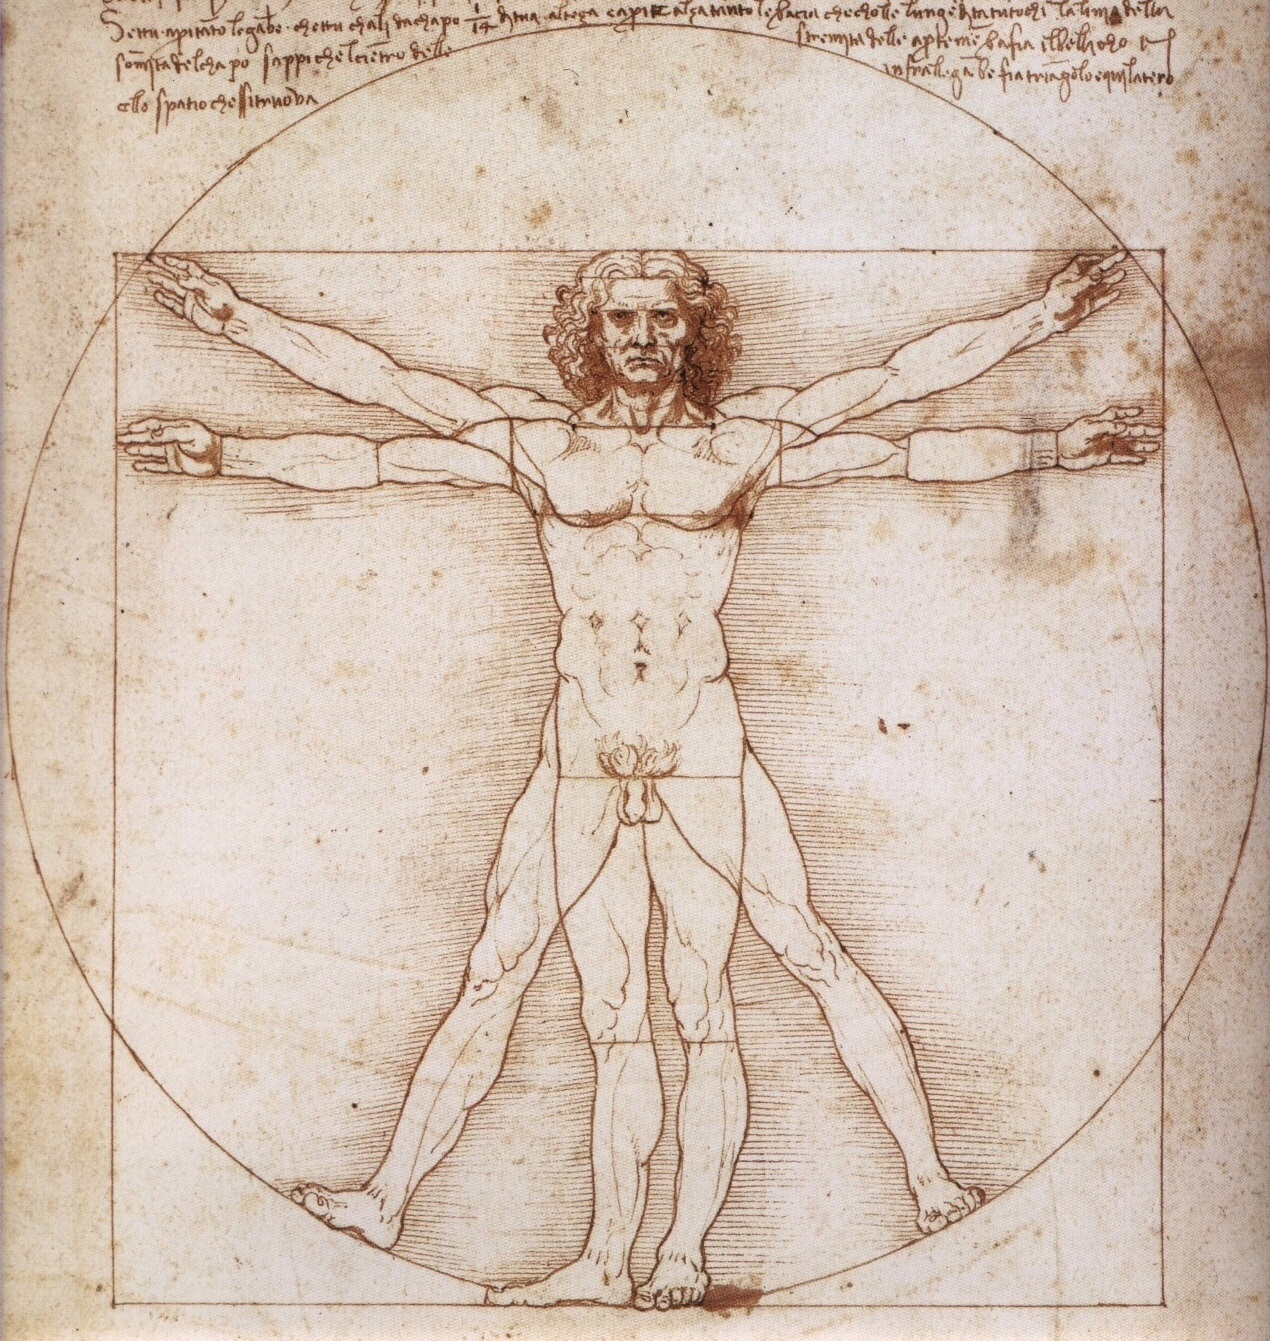
\includegraphics[width=\paperwidth]{uomo_vitruviano.jpg}
    };
  \end{tikzpicture}
\end{frame}

\section{Part-Based Model for Object Detection}

\begin{frame}{Part-Based Model}
  \metroset{block=fill}
  \begin{block}{Idea}
    An object is made of a set of specific sub-blocks.
  \end{block}
  \pause
  \begin{block}{Pictorial structure}
    Pictorial structures represent objects by a collection of parts arranged in
    a deformable configuration.
  \end{block}
\end{frame}


\begin{frame}{Pictorial Structures}
  \centering
  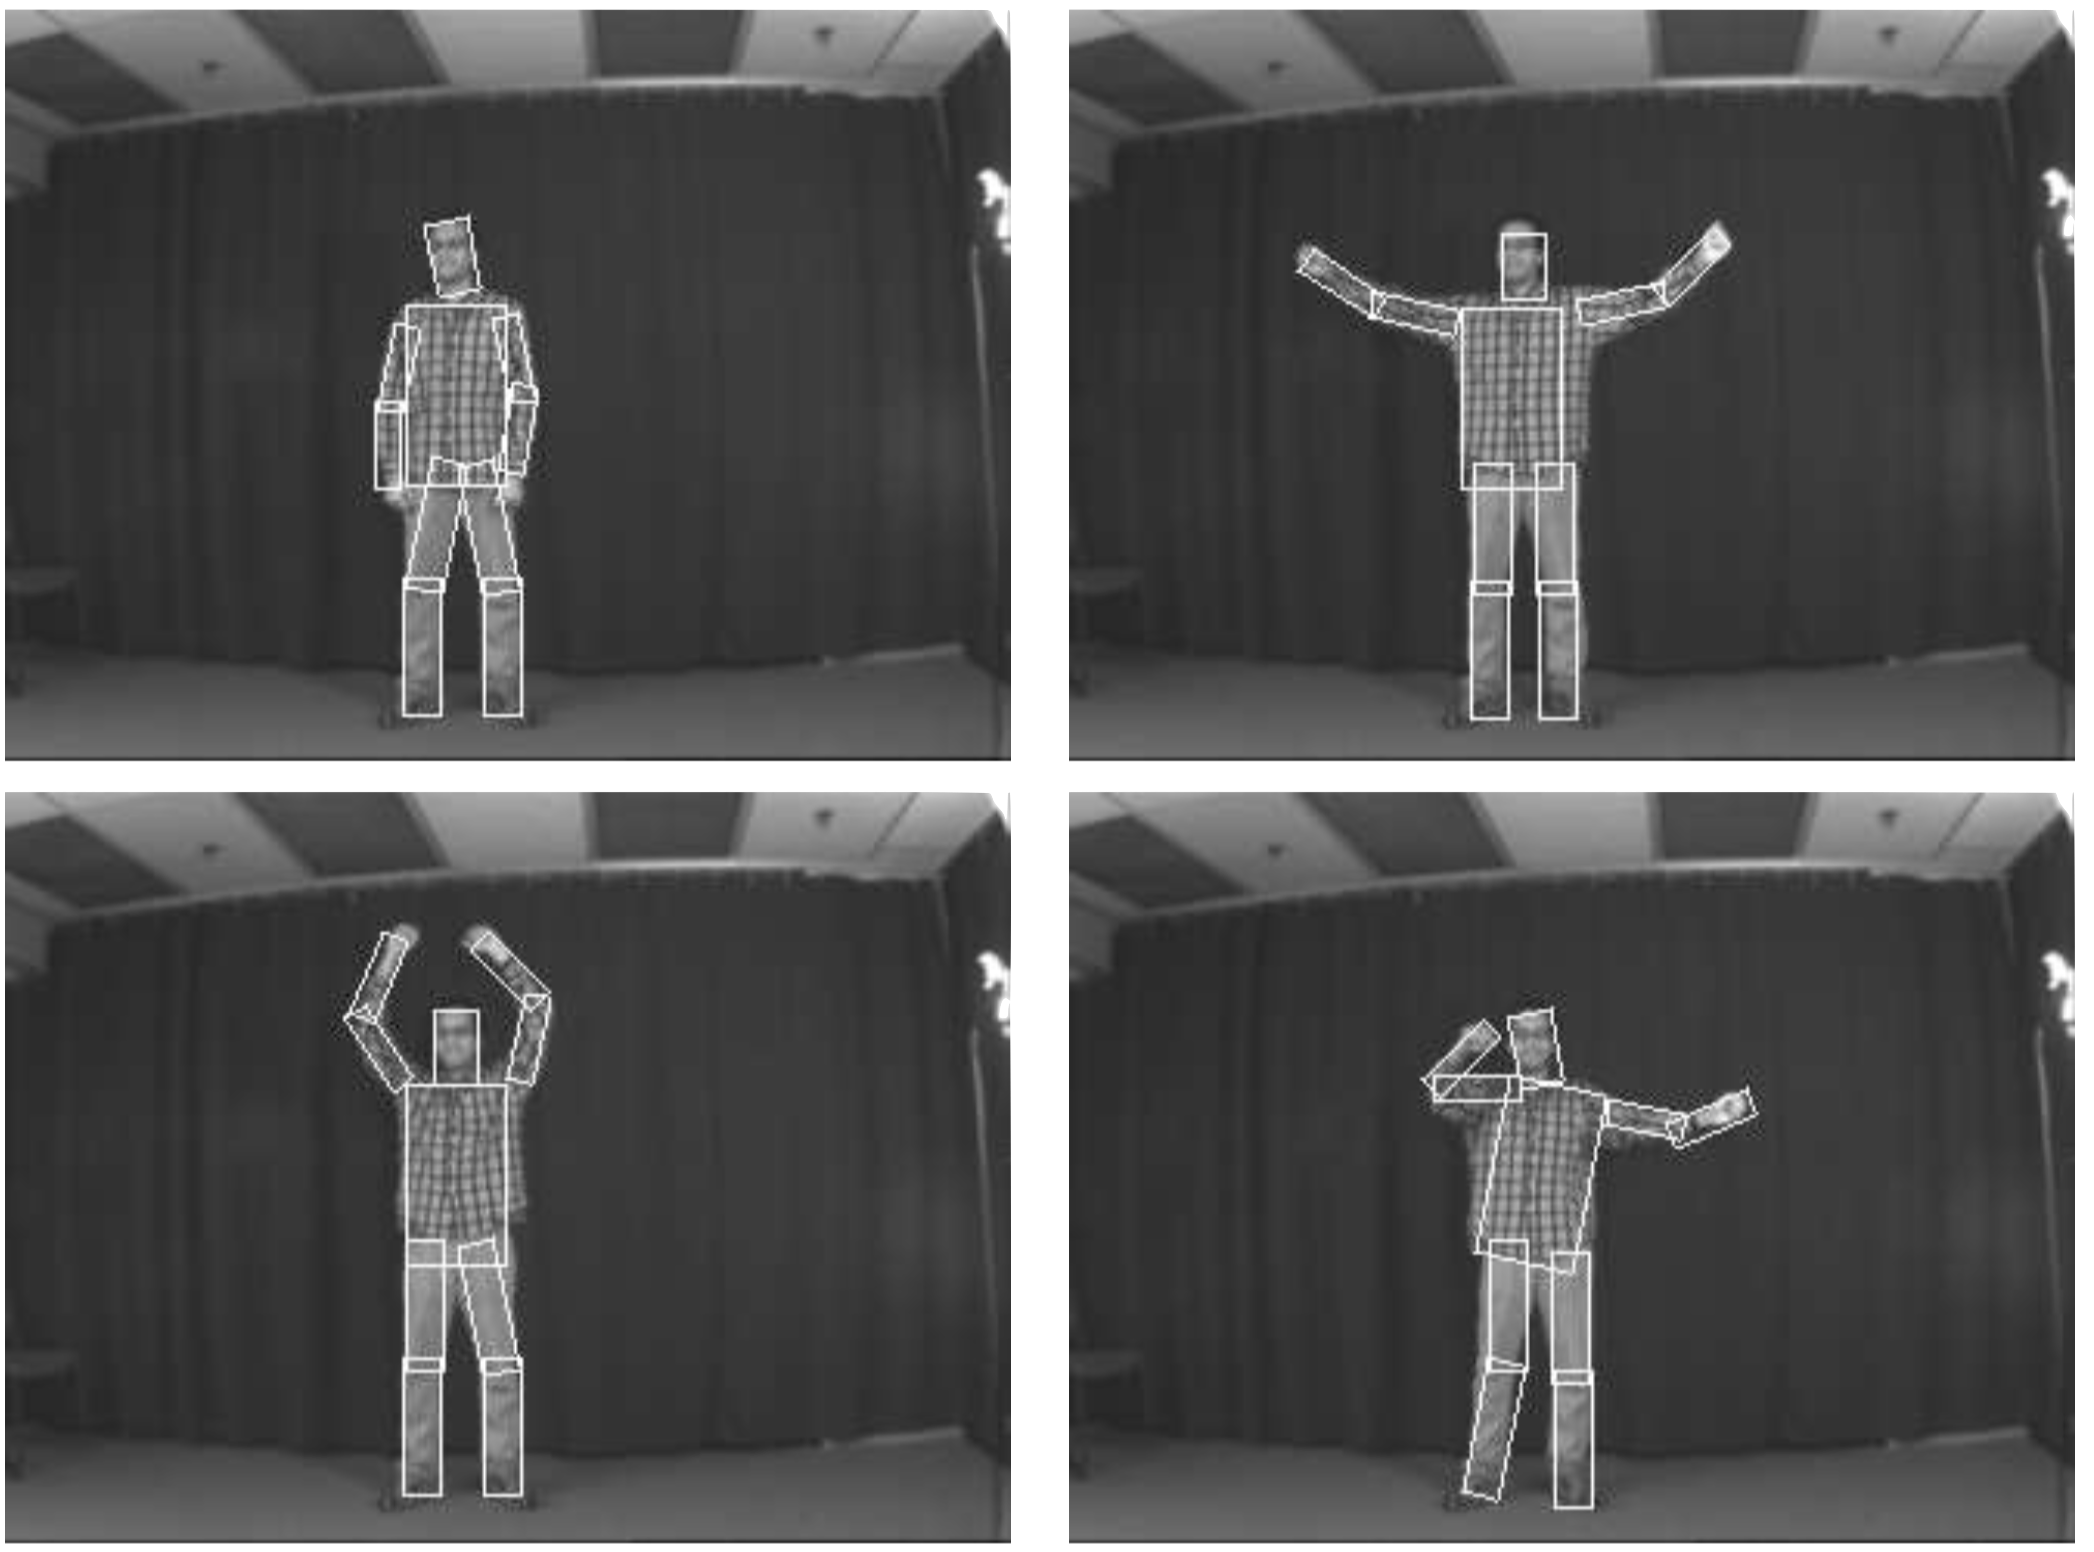
\includegraphics[width=.95\textwidth]{pictorial_structures.png}
\end{frame}
